\documentclass[12pt, a4paper]{article}
\usepackage[francais]{babel}
\usepackage{caption}
\usepackage{graphicx}
\usepackage[T1]{fontenc}
\usepackage{listings}
\usepackage{geometry}
\usepackage{minted}
\usepackage{array,multirow,makecell}
\usepackage[colorlinks=true,linkcolor=black,anchorcolor=black,citecolor=black,filecolor=black,menucolor=black,runcolor=black,urlcolor=black]{hyperref}
\setcellgapes{1pt}
\makegapedcells
\usepackage{fancyhdr}
\pagestyle{fancy}
\lhead{}
\rhead{}
\chead{}
\rfoot{\thepage}
\lfoot{Martin Baumgaertner}
\cfoot{}
\renewcommand{\footrulewidth}{0.4pt}
\renewcommand{\headrulewidth}{0.4pt}
\renewcommand{\listingscaption}{Code}
\renewcommand{\listoflistingscaption}{Table des codes}
% \usepackage{mathpazo} --> Police à utiliser lors de rapports plus sérieux

\begin{document}
\begin{titlepage}
	\newcommand{\HRule}{\rule{\linewidth}{0.5mm}} 
	\center 
	\textsc{\LARGE iut de colmar}\\[1.5cm] 
	\textsc{\Large R301}\\[0.5cm] 
	\textsc{\large Année 2022-23}\\[0.5cm]
	\HRule\\[0.75cm]
	{\huge\bfseries Réseaux de campus}\\[0.4cm]
	\HRule\\[1.5cm]
	\textsc{\large martin baumgaertner}\\[0.5cm] 

	\vfill\vfill\vfill
	{\large\today} 
	\vfill
\end{titlepage}
\newpage
\tableofcontents
\newpage
\section{CM 1 - 5 septembre 2022}
\subsection{Les technologies sans fils}
\begin{itemize}
    \item WPAN (Wireless Personal Area Network) : réseau sans fil de petite portée (10m) entre des appareils mobiles (téléphones, ordinateurs portables, etc.). Exemples : Bluetooth, ZigBee, etc.\\
    \item WMAN (Wireless Metropolitan Area Network) : réseau sans fil de moyenne portée (1km) entre des appareils mobiles (téléphones, ordinateurs portables, etc.). Exemples : Wi-Fi, WiMax, etc.\\
    \item WLAN (Wireless Local Area Network) : réseau sans fil de grande portée (10km) entre des appareils mobiles (téléphones, ordinateurs portables, etc.). Exemples : Wi-Fi, WiMax, etc.\\
    \item WAN (Wide Area Network) : réseau sans fil de très grande portée (100km) entre des appareils mobiles (téléphones, ordinateurs portables, etc.). Exemples : Wi-Fi, WiMax, etc.\\
\end{itemize}

\subsection{Organisme régulateurs}

\begin{itemize}
    \item Wifi alliance = consortium industriel qui possède la marque Wifi.
    \item IEE = Institute of Electrical and Electronics Engineers.
\end{itemize}
\newpage
\subsection{Portée du signal}

\begin{itemize}
    \item 2,4 GHz (802.11 b/g/n) : 70m en intérieur
    \item 5 GHz (802.11 n/ac/ax) : 35m en intérieur 
    \item 6 Ghz (802.11 be) : 30m en général \\
\end{itemize}

En gros, on peut retenir que quand la fréquence diminue, le débit diminue mais
la portée augmente. 

\begin{figure}[H]
    \centering
    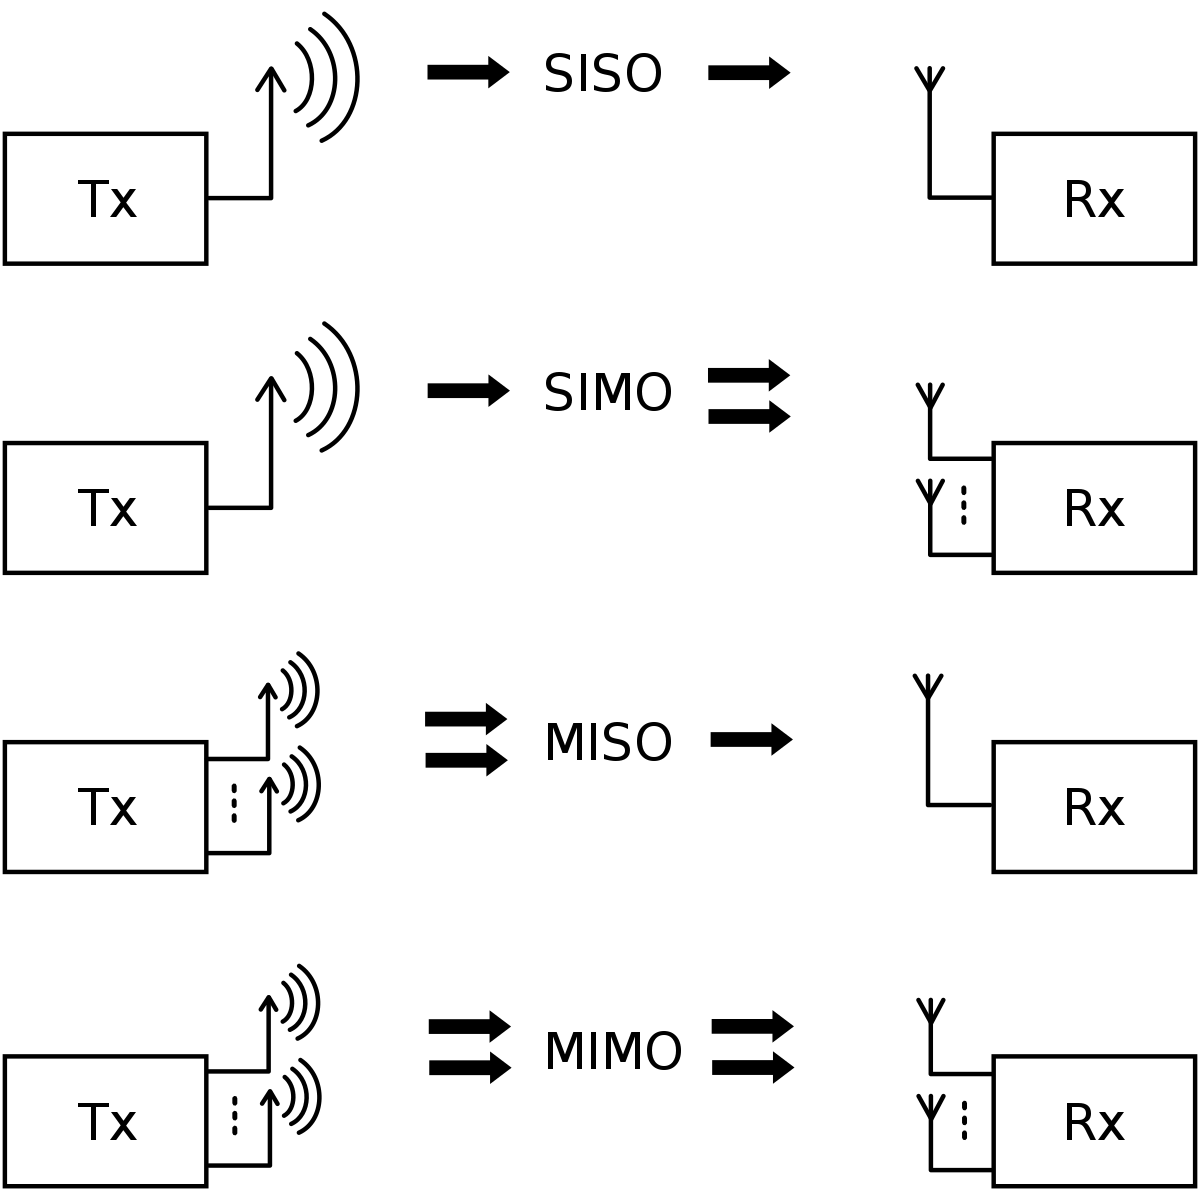
\includegraphics[width=0.5\textwidth]{img/rx.png}
    \caption{Réception d'un signal}
    \label{fig:schema}
\end{figure}

\subsection{Rappel collisions et intrerférences}
Collisons = sur un meme canal gégrées par un algorithme. 

\subsection{Bande ISM}
Les canaux 12 et 13 sont quasi interdits aux USA sauf à faire puissance le 14 étant
strictement interdit dans le pays.

\subsection{Les topologies de base}
Avec point d'accès = la borne n'est pas barrée\\
Sans point d'accès = la borne est barrée

\subsection{Mode infrasctucture}
ESSID/SSID : nom du réseau\\
Un AP configuré dans ce mode va jouer le rôle de simple carte WIFI, via le câble 
ethernet. 
\subsection{Mode répéteur (repeaters)}
\begin{itemize}
    \item Sert à étendre le réseau dans des zones d'ombres
    \item Débit divisé par 2
    \item Risque de collision élevé car c'est sur la même fréquence
\end{itemize}

\subsection{Sécuriser son réseau}
\begin{itemize}
    \item WEP : Wired Equivalent Privacy (déjà obsolète), très facile à pirater
    \item WPA : Wi-Fi Protected Access, plus sécurisé que WEP, solution transitoire 
    \item conçue avant la finalisation de la norme 801.11i
    \item WPA2 : Wi-Fi Protected Access 2, plus sécurisé que WPA, respecte a norme 
    \item 802.11i et imposee le protocole de gestion de cles CCMP
    \item WPA3 : Wi-Fi Protected Access 3, plus sécurisé que WPA2, introduit en 2018
    \item WPA Personal : WPA avec une seule clé partagée par tous les utilisateurs, conçue pour les petits réseaux 
    \item WPA entreprise : WPA avec une clé différente pour chaque utilisateur, conçue pour les grands réseaux d'entreprise\\
\end{itemize}

Voici quelques solution pour sécurer son réseau : \\
\begin{itemize}
    \item Cacher le SSID
    \item Filtrer adresses MAC
    \item Utiliser le WPA3
\end{itemize}

\subsection{Pirater son réseau}
\begin{itemize}
    \item Utiliser Macchanger pour changer adresse MAC
    \item utiliser airodump-ng pour les stations disponibles
    \item utiliser aireplay-ng pour envoyer une trame de déconnexion d'une station connectéé, qui va alors tenter de se reconnecter automatiquement
    \item Utiliser AirCrack-ng avec un fichier adéquat
\end{itemize}


\end{document}